\chapter{System Evaluation}
This chapter evaluates the system, analysing the various aspects of the project 
to ensure the requirements of the project were met and discusses the various 
types of testing that was performed throughout the software development cycle to
ensure each of the requirements was met and the software was of high quality. 

\section{Overview}
The system was designed and developed using the Test Driven Development (TDD) 
methodology. As each unit of code was written and before each new component was 
integrated into the system, appropriate tests were carried out and adjusted if 
needed. Because of this, a lot of bugs were caught early on, allowing them to be
fixed with minimal disruption to the system as a whole. This also allowed the 
system to be redesigned early on when necessary.

\par
\bigskip
The types of testing carried out were as follows:

\begin{itemize}
    \item End-to-End Testing
    \item Exploratory Testing
    \item Functional Testing
    \item Graphical User Interface (GUI) Testing
    \item Integration Testing
    \item Unit Testing
    \item System Testing
\end{itemize}

\section{End-to-End Testing}
\begin{center}
    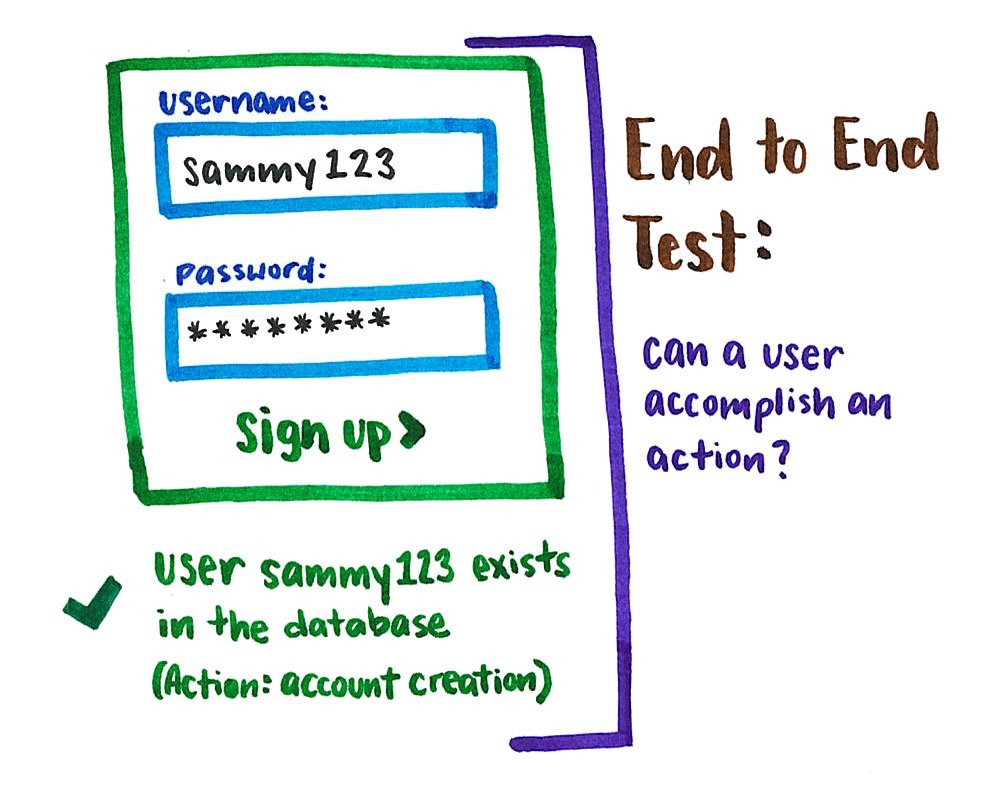
\includegraphics[width=6cm,height=10cm,keepaspectratio]{images/e2e_1}
    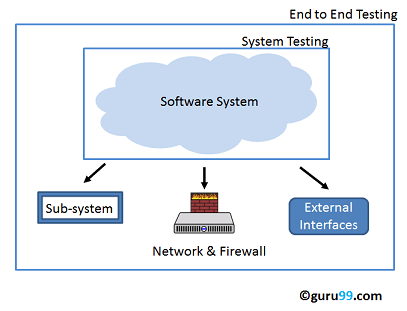
\includegraphics[width=6cm,height=10cm,keepaspectratio]{images/e2e_2}
\end{center}

End-to-end testing is a technique used to test whether the flow of an 
application right from start to finish is behaving as expected. The purpose of 
performing end-to-end testing is to identify system dependencies and to ensure
that the data integrity is maintained between various system components and 
systems.

\par
\bigskip

The entire application is tested for critical functionalities such as 
communicating with the other systems, interfaces, database, network, and other 
applications. 

\section{Exploratory Testing}
\begin{center}
    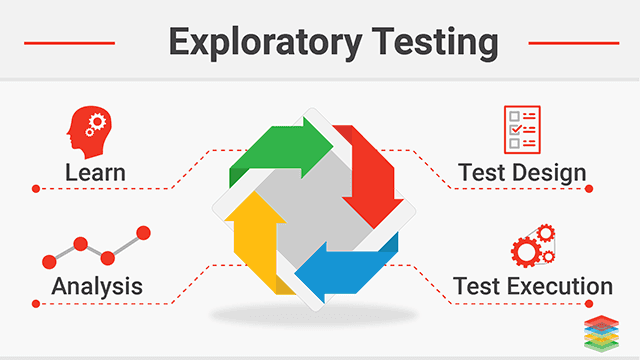
\includegraphics[width=12cm,height=10cm,keepaspectratio]{images/xenonstack-what-is-exploratory-testing}
\end{center}
Exploratory testing is a technique or a method whose aim is to discover the
flaws during the process of software development. 

\par
\bigskip

This technique of testing is concerned about the qualitative assurance of the 
software. It is used to discover the anonymous issues during the process of 
development of software. 

\section{Functional Testing}
\begin{center}
    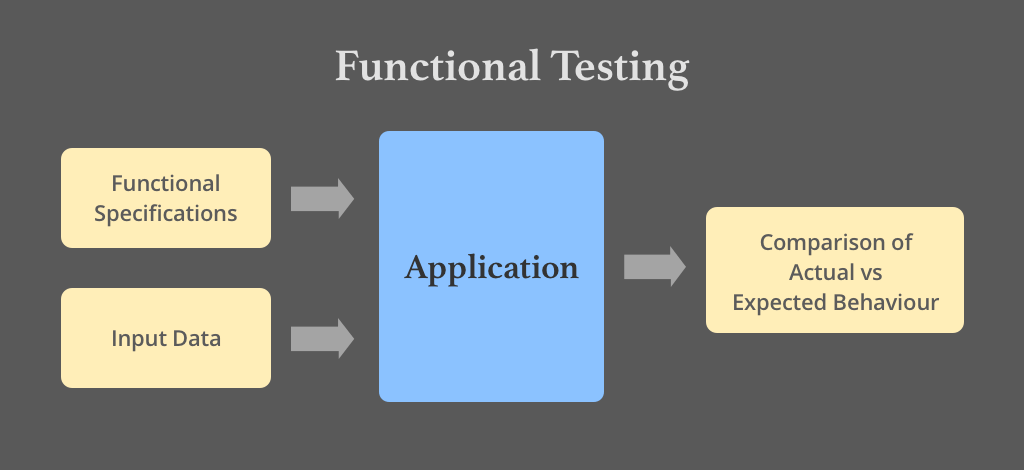
\includegraphics[width=12cm,height=10cm,keepaspectratio]{images/Functional-Testing-feature-image}
\end{center}
Functional Testing is a type of software testing whereby the system is tested 
against the functional requirements/specifications.

\par
\bigskip

Functions (or features) are tested by feeding them input and examining the 
output. Functional testing ensures that the requirements are properly satisfied 
by the application. This type of testing is not concerned with how processing 
occurs, but rather, with the results of processing. It simulates actual system 
usage but does not make any system structure assumptions.

\par
\bigskip

During functional testing, Black Box Testing technique is used in which the 
internal logic of the system being tested is not known to the tester.

\subsection{Web Application}


\section{Graphical User Interface (GUI) Testing}
\begin{center}
    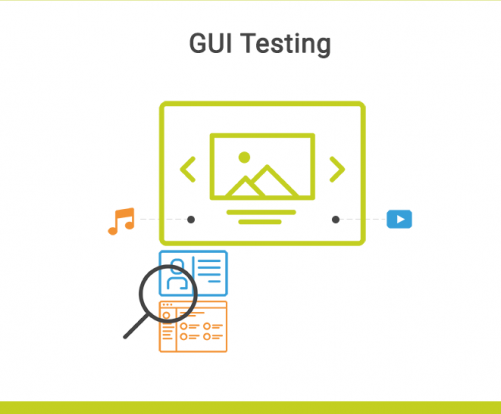
\includegraphics[width=12cm,height=10cm,keepaspectratio]{images/gui_testing}
\end{center}
Graphical User Interface (GUI) Testing is a software testing type that checks
the Graphical User Interface of the Application Under Test. GUI Testing involves
checking the screens with the controls like menus, buttons, icons, and all types
of bars - toolbar, menu bar, dialog boxes, and windows, etc. The purpose of GUI 
Testing is to ensure UI functionality works as per the specification.

\section{Integration Testing}
\begin{center}
    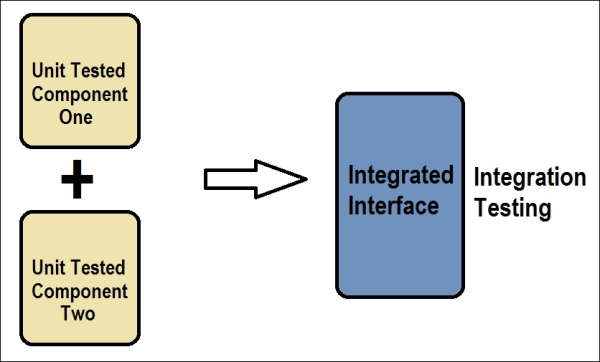
\includegraphics[width=12cm,height=10cm,keepaspectratio]{images/integration}
\end{center}
Integration testing (sometimes called integration and testing, abbreviated I&T) 
is the phase in software testing in which individual software modules are 
combined and tested as a group. Integration testing is conducted to evaluate the
compliance of a system or component with specified functional requirements.

\section{Unit Testing}
\begin{center}
    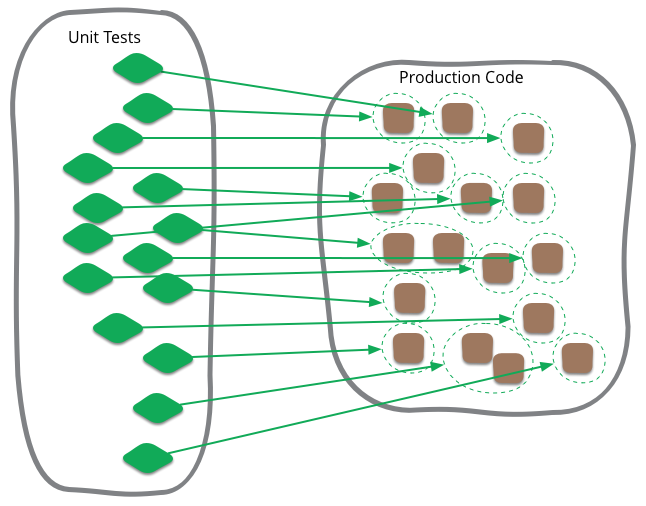
\includegraphics[width=12cm,height=10cm,keepaspectratio]{images/unit}
\end{center}
Unit Testing is a level of software testing where individual units/ components
of a software are tested. The purpose is to validate that each unit of the
software performs as designed. A unit is the smallest testable part of any 
software. It usually has one or a few inputs and usually a single output.

\section{System Testing}
\begin{center}
    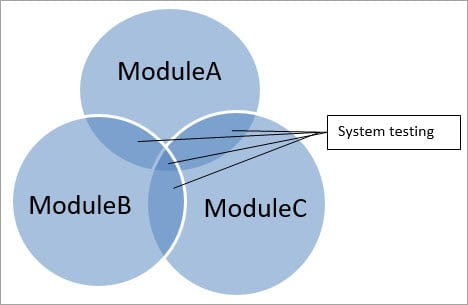
\includegraphics[width=12cm,height=10cm,keepaspectratio]{images/system-testing-example}
\end{center}
System Testing is a level of testing that validates the complete and fully
integrated software product. The purpose of a system test is to evaluate the 
end-to-end system specifications. Usually, the software is only one element of a
larger computer-based system. Ultimately, the software is interfaced with other 
software/hardware systems.